\section{Durchführung}
\label{sec:Durchführung}

\subsection{Versuchsaufbau}
Für den Versuch wird der in \autoref{fig:Aufbau} dargestellte Aufbau verwendet.
Die wesentlichen Bestandteile gehen aus der Theorie hervor, der verwendete Kondensator
ist mit einem Schalter verbunden, sodass die Spannung zügig umgekehrt oder abgeschaltet werden kann.
Über dem Kondensator befindet sich eine Öffnung, durch die mit einem Zerstäuber Öltröpchen
gesprüht werden können.
Sollte deren Ladung zu gering sein, können diese mithilfe eines leicht radioaktiven $\alpha$-Präparates (hier Thorium)
ionisiert werden, um die Ladung zu erhöhen.
Eine Halogenlampe beleuchtet die Öltröpchen sowie den Kondensator von innen, an dessen Rückseite ist ein Gitter aufgezeichnet.
Mit einem Mikroskop schaut man von Vorne in den Kondensator und beobachtet die Bewegung der Öltröpchen vor dem Gitter,
sodass deren Geschwindigkeit ermittelt werden kann.
Die Spannung am Kondensator sowie die darin herschende Temperatur können mithilfe von zwei angeschlossenen Multimetern
gemessen werden, die Temperatur wird dabei indirekt über einen Widerstand bestimmt.
\begin{figure} [H]
    \centering
    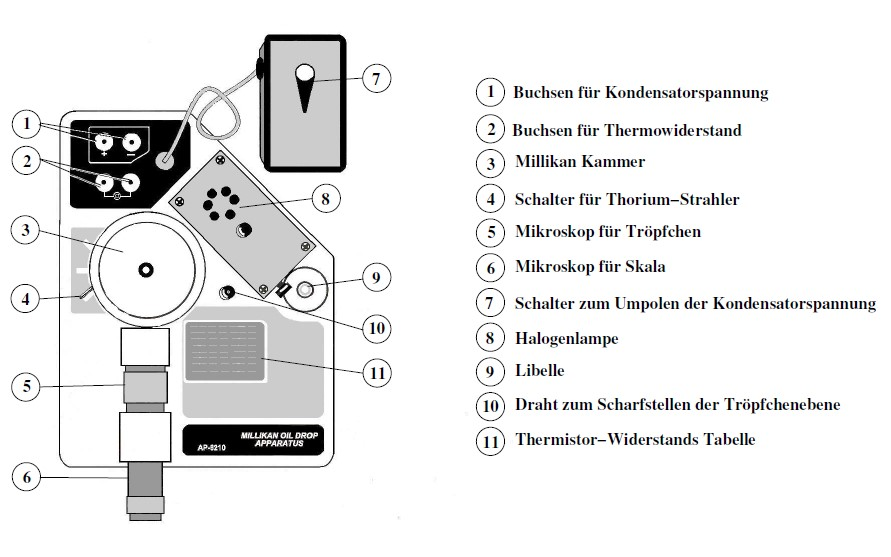
\includegraphics[height=6cm]{content/pics/Aufbau.jpg}
    \caption{Versuchsaufbau mit Beschriftung \cite{v503}.}
    \label{fig:Aufbau}
\end{figure}

\subsection{Messung der Geschwindigkeiten}
Insgesamt werden fünf Messreihen durchgeführt, die bis auf die Ausgangsparameter alle identisch sind.
Für die erste Messreihe wird eine Kondensatorspannung von $U=\qty{150}{\volt}$ eingestellt sowie der temperaturabhängige
Widerstand gemessen.
Es werden nun Öltröpfchen in den Kondensator gesprüht und deren Verhalten bei aktiviertem E-Feld beobachtet.
Sollte die Bewegung zu langsam sein, werden die Tröpfchen kurz bestrahlt, um die Ladung zu erhöhen.
Nachdem ein gut sichtbares Tröpfchen ausgewählt wurde, kann mit der Messung begonnen werden.
Es werden die Geschwindigkeiten $v_{\symup{auf}}$ und $v_{\symup{ab}}$ bestimmt, indem die Zeit gemessen wird,
die dieses Tröpfchen zum Zurücklegen einer festgelegten Strecke zwischen zwei Linien des Gitters benötigt.
Hierfür wird das elektrische Feld mittels des Schalters aktiviert und die Richtung jeweils hin und her gewechselt.
Diese Messung wird drei mal wiederholt, anschließend wird noch die Fallgeschwindigkeit $v_0$ des selben Tröpfchens gemessen.
Dieses Vorgehen wird für vier weitere Öltröpfchen wiederholt.

Bei den vier weiteren Messreihen wird jediglich die Kondensatorspannung variiert, hierfür wird die ursprüngliche
Spannung pro Messreihe um $\symup{\Delta}U=\qty{25}{\volt}$ erhöht.